\section{Administrative Area}
The Administrative processes are performed by the gorup of employee grouped in the Admnistrative Organizational unit according to the Working Structure in figure \ref{2img:wstruct}. In particular all the processes are supervised by the CEO who is the leader of the organizational's trend.


\subsection{Billing}
This process provides support for the definition of the appropriate
remuneration for the service supplied.
The process takes into account the history of project development and the details defined in the contract, in order to check if they match or if some extra features have been during the development phase. The employees mainly involved are Business Consultant, Secretary and the CEO.

Image \ref{2img:billing} shows how this process is realized in practice, focusing on the resources used and the targets for each activity. The goal of this process is to provide a fair billing to the customer, balanced on the services actually delivered.

\begin{figure}[ht!]
\begin{centering}
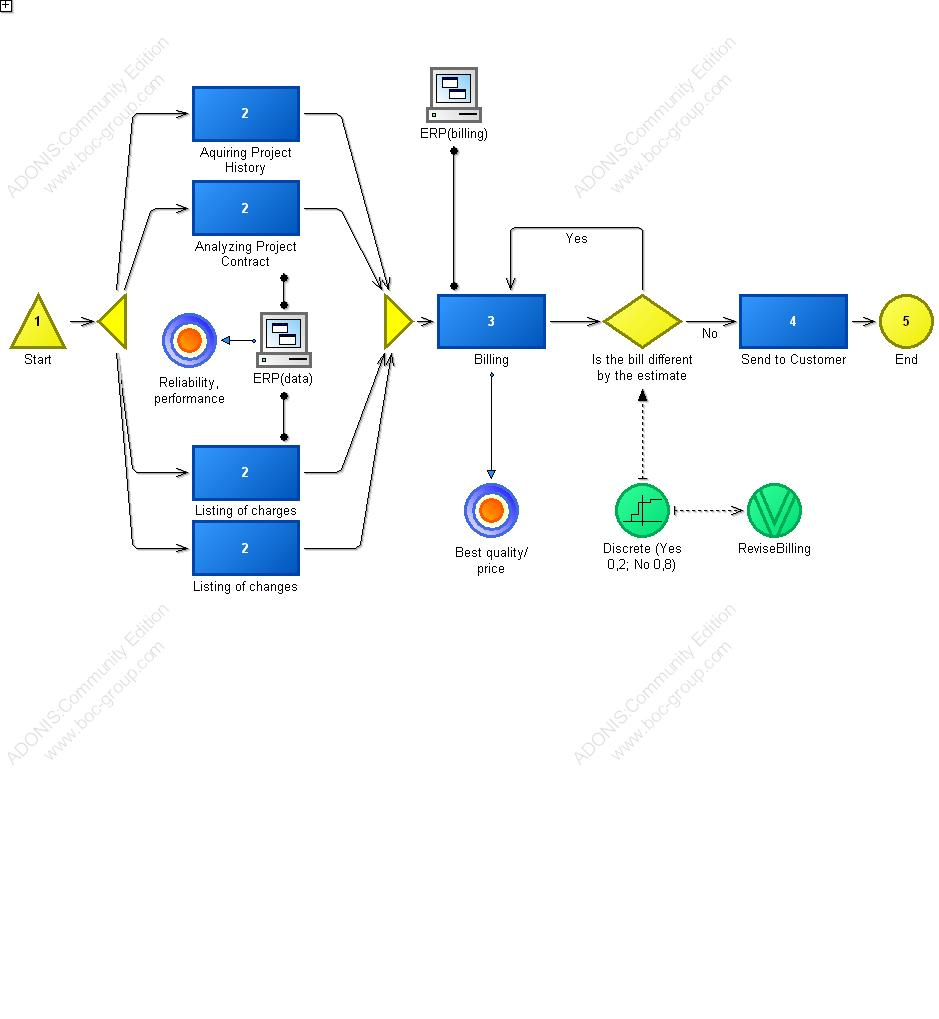
\includegraphics[scale=0.50, angle=90]{assign2/adonis/imgs/billing.jpg}
\caption{AllSparks billing process.}
\label{2img:billing}
\end{centering}
\end{figure}

\emph{Path Analysis}\\
The analysis of possible paths results five correspondence, one with the 82,30\% of probability to be performed. For simulation's convention the number of these processes per month is configured on three element on average.

\begin{alltt}
Probability:   79,9000%
Execution time:  00:000:00:24:20
Waiting time:  00:000:00:05:00
Resting time:  00:000:00:11:10
Transport time:  00:000:00:01:00
Cycle time:  00:000:00:29:20
Costs:  0,000000

Billing 0.2 (Business process model)
========================================
Process start: Start
Parallelity: Parallelity-25245
    *
    Activity: Aquiring Project History
    *
    Activity: Analyzing Project Contract
    *
    Activity: Listing of charges
    *
    Activity: Listing of changes
Merging: Merging-25248
Activity: Billing
Decision: Is the bill different by the estimate --> ReviseBilling = 'No'
Activity: Send to Customer
End: End
\end{alltt}

\emph{Capacity Analysis}\\
The capacity analysis of the process illustrates the specified timing and costs forseen for the single activities. Morevover it exlicities the Performer associated to each activity in order to check the responsibility for each step of the Business Process.

\begin{landscape}
{\tiny
\begin{tabular}{|l|l|l|l|l|l|l|}
Business process&Activity&Performer&Number&Execution time&Cycle time&Costs\\
\hline
Billing 0.3&&&&00:000:00:24:51&00:000:00:32:42&33,575000\\
\hline
&Aquiring Project History (Billing 0.3)&&1,000000&00:000:00:10:00&&1,300000\\
\hline
&&Secretary (AllSpark - Working Environment 0.1)&1,000000&00:000:00:10:00&&1,300000\\
\hline
&Analyzing Project Contract (Billing 0.3)&&1,000000&00:000:00:10:00&&0,200000\hline
\hline
&&Secretary (AllSpark - Working Environment 0.1)&1,000000&00:000:00:10:00&&0,200000\\
\hline
&Listing of charges (Billing 0.3)&&1,000000&00:000:00:01:00&&0,300000\\
\hline
&&Business consultant (AllSpark - Working Environment 0.1)&1,000000&00:000:00:01:00&&0,300000\\
\hline
&Billing (Billing 0.3)&&1,259000&00:000:00:02:31&&31,475000\\
\hline
&&Business consultant (AllSpark - Working Environment 0.1)&1,259000&00:000:00:02:31&&31,475000\\
\hline
&Listing of changes (Billing 0.3)&&1,000000&00:000:00:01:00&&0,200000\\
\hline
&&Secretary (AllSpark - Working Environment 0.1)&1,000000&00:000:00:01:00&&0,200000\\
\hline
&Send to Customer (Billing 0.3)&&1,000000&00:000:00:00:20&&0,100000\\
\hline
&&Secretary (AllSpark - Working Environment 0.1)&1,000000&00:000:00:00:20&&0,100000\\
\hline
&Total&&&&00:000:00:24:51&&33,575000
\end{tabular}
}
\end{landscape}
%

%

\paragraph{Bureaucracy Management}
\paragraph{Financial support}
\paragraph{Marketing Management}
\paragraph{Public Relation Management}
